\documentclass{article}
\usepackage[utf8]{inputenc}
\usepackage[legalpaper, margin=1in]{geometry}
\usepackage{listing}
\usepackage{graphicx}
\usepackage{float}
\usepackage{listings}


\title{Signals and Systems - Rate Change}
\author{Mazz Shaikh - 932056724\\ Ron Abraham - }

\begin{document}

\maketitle

\section*{Part 1}
\subsection*{1}
\subsection*{2}

\newpage
% ---------------------------------------------------------------------------
% ------------------------------- Part 1 ------------------------------------
% ---------------------------------------------------------------------------

\section*{Part 2}
% ------------------------------- Section 1 ----------------------------------

\subsection*{1}

\begin{figure}[H]
    \centering
    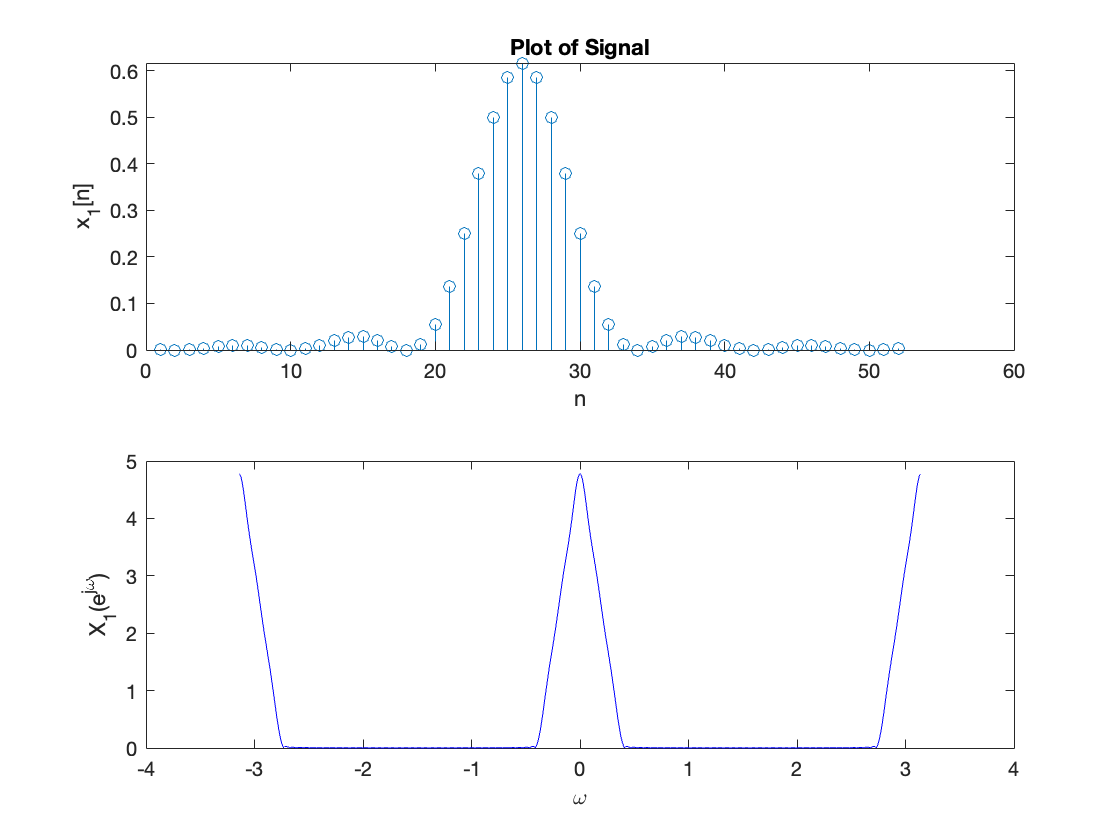
\includegraphics[scale=0.4]{Plot of Signal.png}
    \caption{Plot of Signal}
    \label{Plot of Signal}
\end{figure}
% ------------------------------- Section 2 ----------------------------------
\subsection*{2}

\begin{figure}[H]
    \centering
    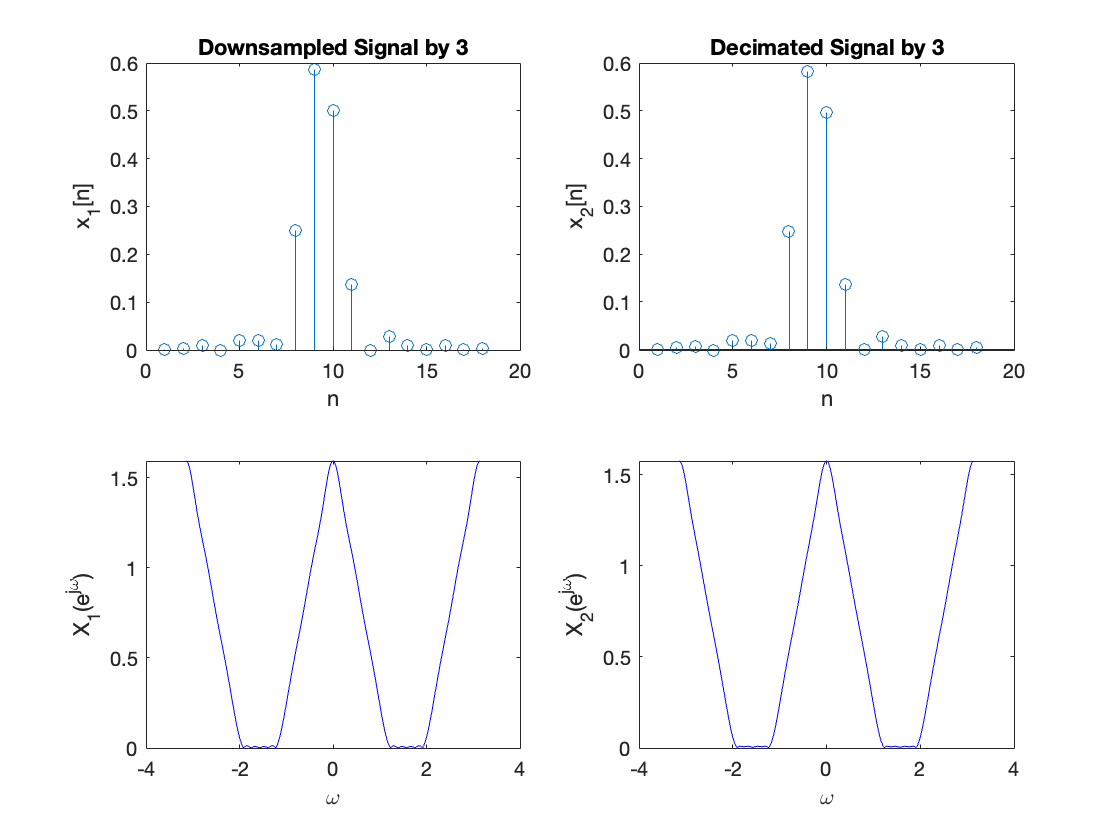
\includegraphics[scale = 0.4]{Downsample 3.png}
    \caption{Downsampling by 3}
    \label{Downsampling by 3}
\end{figure}

There is no significant difference between downsample and decimate. 

% ------------------------------- Section 3 ----------------------------------

\subsection*{3}

\begin{figure}[H]
    \centering
    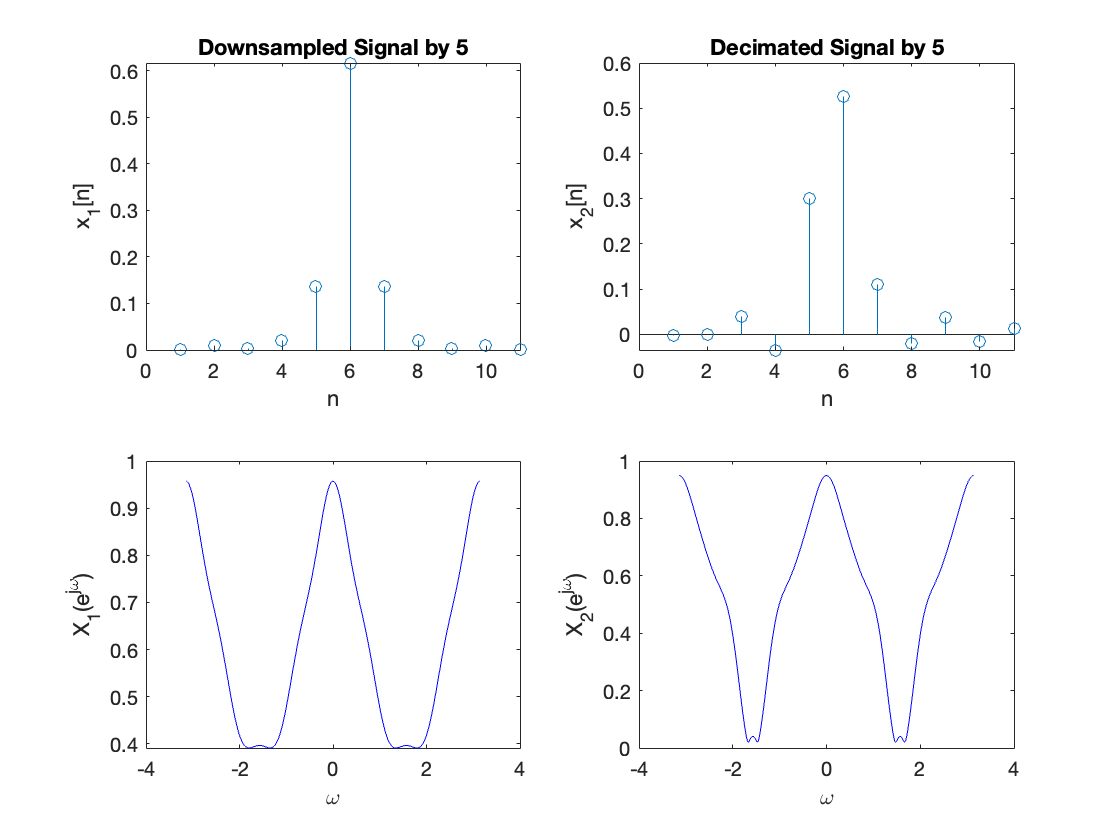
\includegraphics[scale = 0.4]{Downsample 5.png}
    \caption{Downsampling by 5}
    \label{Downsampling by 5}
\end{figure}

% ------------------------------- Section 4 ----------------------------------

\subsection*{4}

\begin{figure}[H]
    \centering
    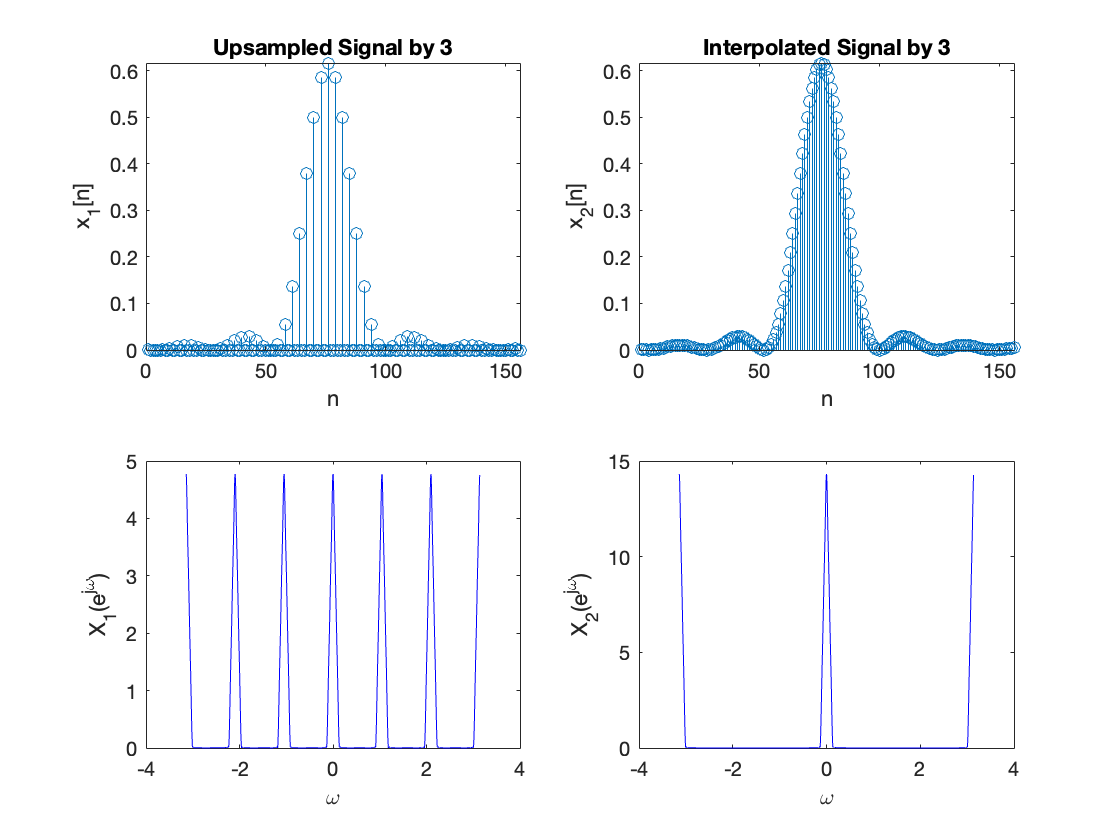
\includegraphics[scale=0.4]{Interpolated 3.png}
    \caption{Interpolated by 3}
    \label{Interpolated by 3}
\end{figure}

% ------------------------------- Section 5 ----------------------------------

\subsection*{5}

\begin{figure}[H]
    \centering
    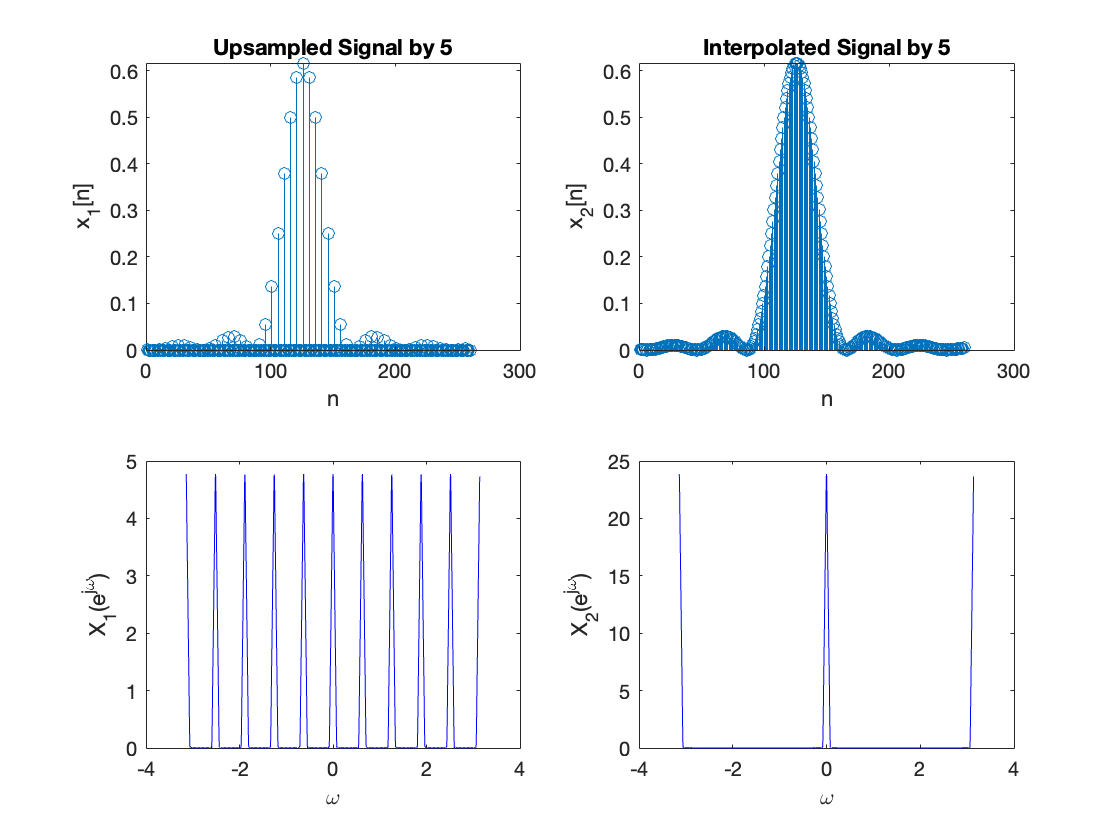
\includegraphics[scale=0.4]{Interpolated 5.png}
    \caption{Interpolated by 5}
    \label{Interpolated by 5}
\end{figure}

% ------------------------------- Section 6 ----------------------------------

\subsection*{6}

\begin{figure}[H]
    \centering
    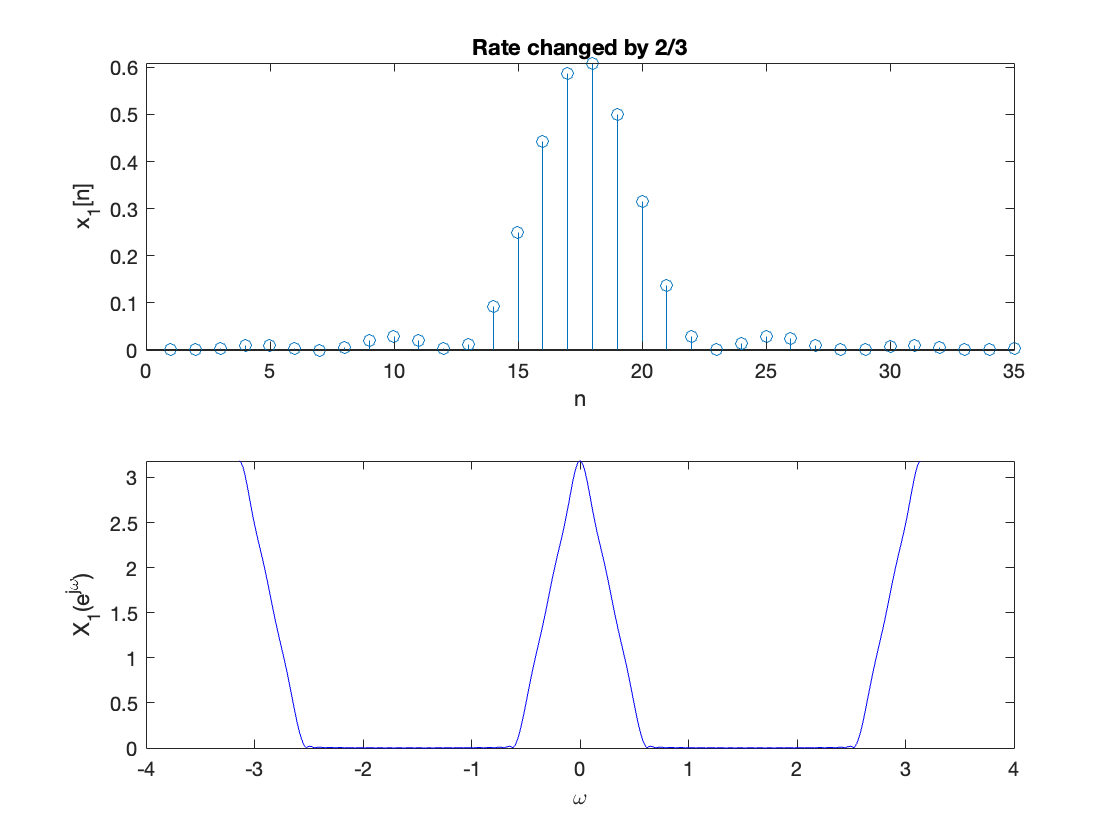
\includegraphics[scale=0.4]{Rate change.png}
    \caption{Interpolated by 3}
    \label{Rate Change}
\end{figure}


\newpage
\section*{Part 3}

\begin{figure}[H]
    \centering
    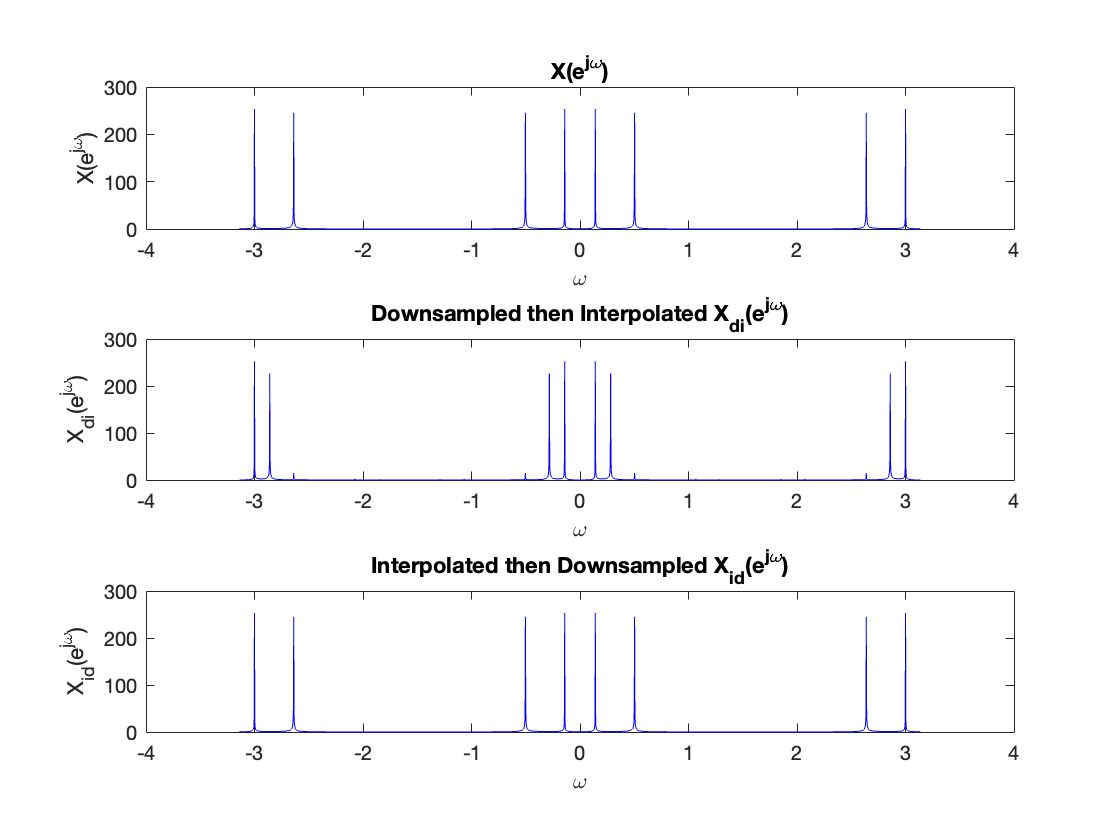
\includegraphics[scale=0.4]{Part 3.png}
    \label{Part 3}
\end{figure}
\end{document}